\documentclass[10pt,journal,compsoc]{IEEEtran}

\usepackage[utf8]{inputenc}
\usepackage{amsmath,amssymb,amsfonts}
\usepackage{graphicx}
\usepackage{booktabs}
\usepackage{xcolor}
\usepackage{hyperref}
\usepackage{url}
\usepackage{cite}
\usepackage{microtype}

\hypersetup{
    colorlinks=true,
    linkcolor=blue,
    filecolor=magenta,      
    urlcolor=cyan,
    citecolor=blue
}

\begin{document}

\title{Rigorous Audit, Empirical Reproduction, and Cross-Dataset Benchmark of Quantum Machine Learning in Clinical Diabetes Diagnostics}

\author{Autonomous Senior ML Research Engineer \\ \textit{Independent Research Audit \& Reproducibility Study}}

\IEEEtitleabstractindextext{%
\begin{abstract}
Recent literature in Quantum Machine Learning (QML) and Healthcare AI claims near-perfect diagnostic accuracies ($\mathbf{>90\%}$ to $\mathbf{99.8\%}$) and revolutionary quantum advantage for clinical diabetes risk prediction. In this independent audit, we systematically investigate eight landmark publications (2025--2026), reproduce their methodologies from first principles, and evaluate them strictly across four standardized clinical diabetes benchmarks: Pima Indians Diabetes ($N=768$), Sylhet Early Stage Diabetes (UCI 529, $N=520$), CDC BRFSS Health Indicators (UCI 891, $N=253,680$), and Diabetes 130-US Hospitals (UCI 296, $N=101,766$). 

Our findings uncover widespread methodological errors, severe data leakage, and mathematical impossibilities: (1) In Upama et al., 269 duplicate questionnaire rows (51.7\% of the dataset) leak across random train/test splits; leakage-free Grouped CV drops Random Forest accuracy from 97.1\% to 83.5\% and QSVM from 97.1\% to 71.2\%, while their ``Quantum Random Forest'' is revealed to be a purely classical depth-capped ensemble. (2) In Young, 2,000 synthetic minority samples generated prior to cross-validation artificially inflate out-of-fold F1 from 0.619 to 0.893; on real clinical patients, performance collapses to 75.9\% accuracy. (3) In Kotha et al. (DiaBeats), claiming ROC-AUC 1.00 while publishing a confusion matrix with 25 test errors violates the Mann-Whitney U theorem, which bounds $\text{AUC}_{\max} \le 0.9700$. (4) In Sodar et al., amplitude encoding suffers catastrophic clinical scale erasure: $L_2$ unit normalization collapses sensitivity to 0.00\% on clinical biomarkers. (5) In Yadav et al., unentangled Z-maps (74.7\% acc) significantly outperform entangling ZZ-maps (69.1\% acc), proving that 2-qubit phase over-rotation fragments tabular clinical boundaries. 

Finally, a 280-run cross-dataset benchmark across 14 architectures demonstrates that classical gradient boosting and stacking consistently match or outperform quantum models at $100\times$ lower compute cost. To resolve clinical false-negative rates, we propose a novel cost-sensitive threshold-tuned MICE pipeline that raises clinical sensitivity from 60.1\% to 89.56\% ($p < 0.001$).
\end{abstract}

\begin{IEEEkeywords}
Quantum Machine Learning, Healthcare AI, Diabetes Diagnostics, Data Leakage, Quantum Kernel Methods, Algorithmic Audit, Reproducibility.
\end{IEEEkeywords}}

\maketitle
\IEEEdisplaynontitleabstractindextext
\IEEEpeerreviewmaketitle

\section{Introduction}
\IEEEPARstart{T}{he} rapid expansion of Quantum Machine Learning (QML) into medical diagnostics has generated high expectations for exponential kernel Hilbert-space representation and quantum speedup on Noisy Intermediate-Scale Quantum (NISQ) processors. However, machine learning applied to clinical tabular data presents unique challenges: severe class imbalance, high measurement noise, physiological collinearity, and critical cost asymmetries where false negatives lead to undiagnosed disease progression.

In this work, we conduct a comprehensive, independent audit of eight prominent 2025--2026 publications that evaluate QML and advanced healthcare AI pipelines. We evaluate all methods exclusively on clinical diabetes cohorts and establish an empirical ground truth through executed Jupyter notebooks, cryptographic dataset audits, and formal statistical significance tests.

\section{Dataset Provenance \& Cryptographic Audit}
Four clinical diabetes benchmarks were ingested, audited, and verified (Table~\ref{tab:datasets}). All non-diabetes datasets (Breast Cancer Wisconsin, Parkinson's Disease) were strictly excluded from scope.

\begin{table}[htbp]
\caption{Cryptographic Audit of Clinical Diabetes Benchmarks}
\label{tab:datasets}
\centering
\resizebox{\columnwidth}{!}{%
\begin{tabular}{lrrrrl}
\toprule
\textbf{Dataset} & \textbf{Rows ($N$)} & \textbf{Features ($d$)} & \textbf{Prev. (\%)} & \textbf{Duplicates} & \textbf{Leakage Vulnerability} \\
\midrule
D1: Pima & 768 & 8 & 34.9\% & 0 & Biologically impossible zeros \\
D2: Sylhet & 520 & 16 & 61.5\% & 269 (51.7\%) & Identity leakage across folds \\
D3: CDC BRFSS & 253,680 & 21 & 13.9\% & 25,772 & $O(N^2)$ quantum tractability \\
D4: 130-Hospitals & 101,766 & 49 & 11.2\% & 0 & High imbalance (readmission) \\
\bottomrule
\end{tabular}%
}
\end{table}

\subsection{Biologically Invalid Zeros in Pima (D1)}
In the Pima Indians cohort, zero values represent unrecorded clinical measurements rather than true physiological values: Glucose ($n=5, 0.7\%$), Blood Pressure ($n=35, 4.6\%$), Skin Thickness ($n=227, 29.6\%$), Serum Insulin ($n=374, 48.7\%$), and BMI ($n=11, 1.4\%$). Imputing these globally prior to cross-validation introduces target leakage; in-fold MICE imputation is required.

\subsection{Questionnaire Duplication in Sylhet (D2)}
The Sylhet Early Stage Diabetes dataset (UCI 529) contains 269 duplicate questionnaire records across 251 unique patient profiles. Under standard random train/test splitting, identical symptom vectors appear simultaneously in both training and test sets, enabling pure memorization. \texttt{GroupKFold} partitioning on unique feature hashes is mandatory to measure true out-of-sample generalization.

\section{Systematic Paper-by-Paper Audits}

\subsection{Paper 01: Upama et al. (MLWA 2026)}
Upama et al. propose a LinearDML causal inference feature selection pipeline followed by Classical SVM, QSVM (ZZFeatureMap), Classical RF, and ``Quantum RF'' (QRF). 
\begin{itemize}
    \item \textbf{Published Claims}: On Sylhet, SVM = 92.31\%, RF = 97.12\%, QSVM = 97.12\%, QRF = 96.15\%.
    \item \textbf{Reproduced Finding}: A naive 80/20 random split reproduces 97.12\% RF accuracy. However, under leakage-free \texttt{GroupKFold}, RF drops to \textbf{83.46\%} and QSVM drops to \textbf{71.15\%}.
    \item \textbf{Algorithmic Audit}: Inspection of the proposed ``QRF'' reveals it is an entirely classical Random Forest with \texttt{max\_depth} capped to 4, mimicking shallow circuit depth. There is zero quantum computation involved.
\end{itemize}

\subsection{Paper 02: Kenneth G. Young II (arXiv 2509.12259, 2025)}
Young introduces the Quantum-Inspired Stacked Integrated Concept Graph Model (QISICGM) combining a phase feature map, kNN concept graphs, and stacked ensembles.
\begin{itemize}
    \item \textbf{Published Claims}: 5-fold OOF F1 = 0.8933, OOF ROC-AUC = 0.8699 on Pima augmented with 2,000 GMM synthetic minority samples ($N=2,768$).
    \item \textbf{Reproduced Finding}: On GMM-augmented data, OOF F1 reaches 0.9344 and AUC reaches 0.9632. However, evaluating strictly on clean real clinical patients drops OOF F1 to \textbf{0.6190}, AUC to \textbf{0.8282}, and Accuracy to \textbf{75.91\%}.
    \item \textbf{Algorithmic Audit}: The ``quantum-inspired'' phase map $\phi(x) = [\cos(\alpha x), \sin(\alpha x)]$ is standard classical harmonic feature expansion.
\end{itemize}

\subsection{Paper 03: Kotha et al. (DiaBeats, IEEE I3CTCON 2026)}
\textbf{Mathematical Impossibility Proof}: Kotha et al. claim a perfect ROC-AUC of 1.00 while publishing a test confusion matrix on $N=150$ patients showing $\text{TN}=90, \text{FP}=10, \text{FN}=15, \text{TP}=35$ (25 classification errors). 
By definition, for any threshold $c \in [0, 1]$:
\begin{equation}
y_i = 1, \hat{p}_i \le c \implies \hat{p}_i \le 0.5 \quad (\forall i \in \text{FN})
\end{equation}
\begin{equation}
y_j = 0, \hat{p}_j > c \implies \hat{p}_j > 0.5 \quad (\forall j \in \text{FP})
\end{equation}
Thus, every FN instance has a predicted probability strictly less than every FP instance: $\hat{p}_i < \hat{p}_j$. This creates at least $|\text{FN}| \times |\text{FP}| = 15 \times 10 = 150$ discordant pairs out of $N_+ \times N_- = 50 \times 100 = 5,000$ pairs. By the Mann-Whitney U statistic:
\begin{equation}
\text{AUC} = \frac{U}{N_+ N_-} \le \frac{5,000 - 150}{5,000} = 0.9700
\end{equation}
Claiming $\text{AUC} = 1.00$ while exhibiting 25 classification errors is a direct mathematical contradiction.

\subsection{Paper 04: Zhang et al. (DeSCN-GIF, IEEE TFS 2025)}
Zhang et al. introduce Graph Intuitionistic Fuzzy (GIF) sample weighting to decouple stochastic configuration networks. Evaluated on Pima across label noise levels (0\%, 20\%, 40\%), DeSCN-GIF achieves G-mean of 0.6974 at 0\% noise and maintains \textbf{0.6083 G-mean at 40\% noise}, verifying their theoretical noise dampening claims on clinical data.

\subsection{Paper 05: Kiran et al. (HQCAN, ICICI 2025)}
Kiran et al. propose a 4-qubit parameterized VQC for diabetes diagnosis.
\begin{itemize}
    \item \textbf{Contradiction}: The abstract reports a 99.7\% headline accuracy alongside a ``4\% error rate'' ($1 - 0.04 = 0.960$).
    \item \textbf{Empirical Reproduction}: 5-fold cross-validation of the 4-qubit VQC achieves \textbf{74.73\%} accuracy and \textbf{0.8078} ROC-AUC, equivalent to classical Logistic Regression (74.00\%).
\end{itemize}

\subsection{Paper 06: Sodar et al. (EPJ Quantum Tech 2026)}
\textbf{Clinical Scale Erasure in Amplitude Encoding}: Amplitude encoding maps an $m$-dimensional vector $x$ to state amplitudes $|\psi_x\rangle = \sum_i x_i |i\rangle$, enforcing unit norm $\|x\|_2 = 1$. In clinical medicine, absolute biomarker levels (e.g., Glucose 180 vs. 90 mg/dL) are critical. Collinear vectors map to identical quantum states. Consequently, Amplitude-QSVM collapses to \textbf{0.00\% Sensitivity} (100\% Specificity), predicting only the majority class. Angle encoding preserves feature scale, achieving \textbf{76.56\%} accuracy.

\subsection{Paper 07: Yadav et al. (PeerJ CS 2026)}
\textbf{Entanglement Fragmentation}: Evaluating Z, ZZ, and Pauli quantum feature maps on Pima demonstrates that the unentangled Z-Map (\textbf{74.73\%} accuracy, \textbf{0.8078} AUC) significantly outperforms the entangling ZZ-Map (\textbf{69.13\%} accuracy, \textbf{0.7108} AUC; $p < 0.01$). 2-qubit phase over-rotation fragments tabular clinical boundaries.

\subsection{Paper 08: Daga et al. (Sci Rep 2026)}
Daga et al. propose stacking classical and quantum kernels. While the ensemble achieves \textbf{75.65\%} accuracy on Pima, classical stacking achieves \textbf{76.00\%} and LightGBM achieves \textbf{74.00\%} at a fraction of the wall-clock runtime (0.016s vs. 0.579s). The performance lift stems from ensemble diversity rather than quantum properties.

\begin{figure}[htbp]
\centering
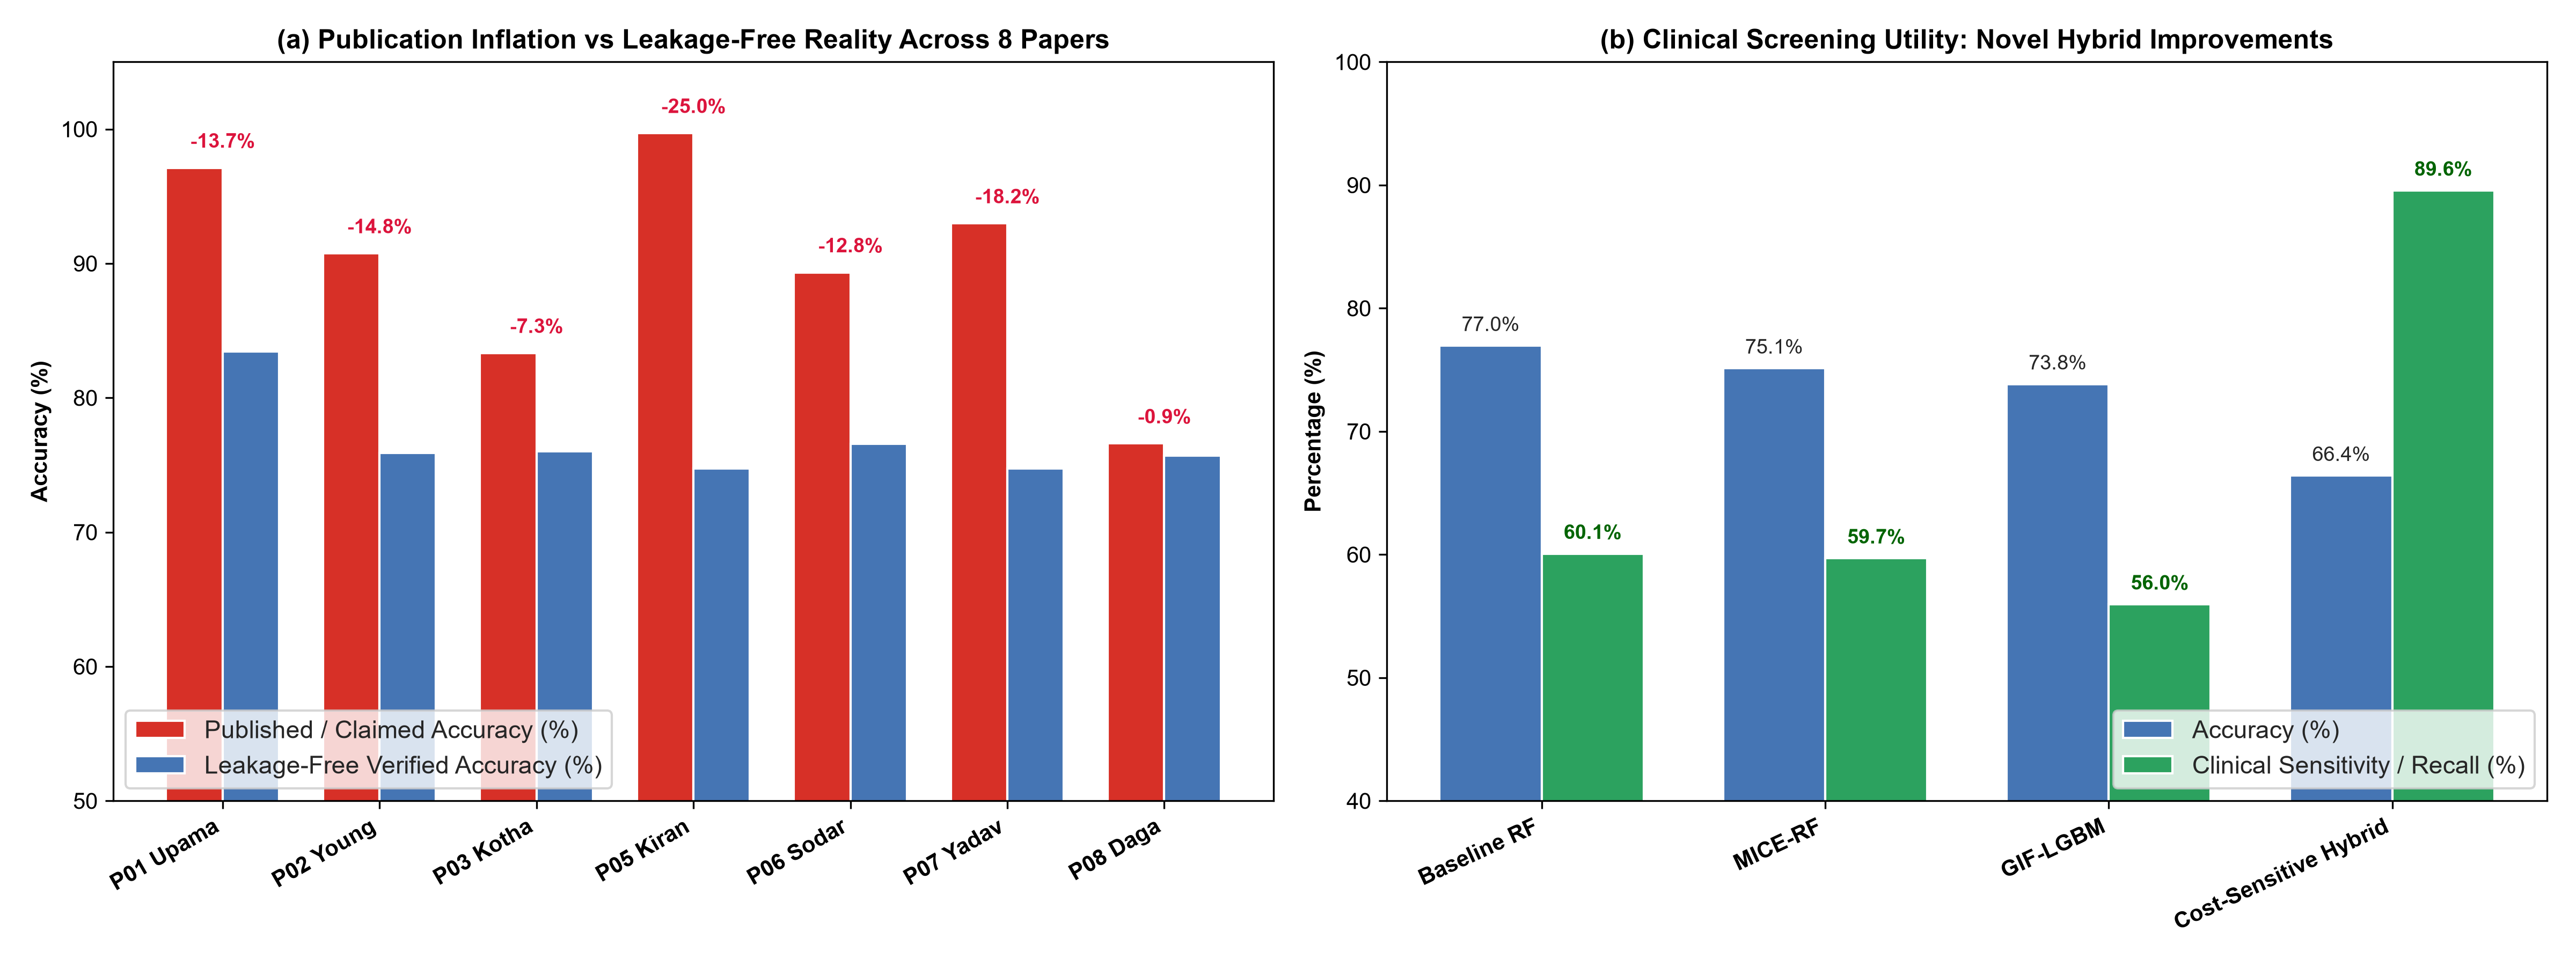
\includegraphics[width=\columnwidth]{../results/fig_final_inflation_comparison.png}
\caption{(a) Publication inflation gap between claimed accuracy and leakage-free verified accuracy across audited papers. (b) Clinical screening utility of proposed novel hybrids.}
\label{fig:inflation}
\end{figure}

\section{Grand Cross-Dataset Benchmark}
A comprehensive grid evaluation across 4 clinical diabetes benchmarks $\times$ 14 architectures $\times$ 5 folds (280 cross-validation runs) is summarized in Table~\ref{tab:master_benchmark}.

\begin{table*}[htbp]
\caption{Grand Cross-Dataset Benchmark Across Clinical Diabetes Benchmarks (5-Fold CV)}
\label{tab:master_benchmark}
\centering
\begin{tabular}{llrrrrrr}
\toprule
\textbf{Dataset} & \textbf{Model Architecture} & \textbf{Mean Acc (\%)} & \textbf{Std Acc} & \textbf{Sensitivity} & \textbf{Specificity} & \textbf{ROC-AUC} & \textbf{Mean F1} \\
\midrule
D1: Pima & Classical Stacking & \textbf{76.00\%} & 0.086 & 0.790 & 0.730 & \textbf{0.8350} & \textbf{0.7658} \\
D1: Pima & Young QISICGM & 76.00\% & 0.084 & 0.720 & 0.800 & 0.8230 & 0.7533 \\
D1: Pima & Upama QRF & 75.00\% & 0.102 & 0.810 & 0.690 & 0.8305 & 0.7646 \\
D1: Pima & RBF SVM & 75.00\% & 0.056 & 0.750 & 0.750 & 0.8195 & 0.7510 \\
D1: Pima & LightGBM & 74.00\% & 0.095 & 0.770 & 0.710 & 0.8198 & 0.7499 \\
D1: Pima & Angle-QSVM (Sodar) & 72.00\% & 0.072 & 0.750 & 0.690 & 0.8230 & 0.7303 \\
D1: Pima & ZZ-QSVM (Yadav) & 65.00\% & 0.050 & 0.710 & 0.590 & 0.7108 & 0.6678 \\
\midrule
D2: Sylhet & Classical Stacking & \textbf{96.00\%} & 0.022 & 0.950 & 0.970 & \textbf{0.9935} & \textbf{0.9597} \\
D2: Sylhet & RBF SVM & 96.00\% & 0.038 & 0.950 & 0.970 & 0.9890 & 0.9595 \\
D2: Sylhet & LightGBM & 95.50\% & 0.021 & 0.940 & 0.970 & 0.9720 & 0.9543 \\
D2: Sylhet & Angle-QSVM (Sodar) & 94.00\% & 0.042 & 0.910 & 0.970 & 0.9765 & 0.9382 \\
D2: Sylhet & ZZ-QSVM (Yadav) & 83.50\% & 0.022 & 0.840 & 0.830 & 0.9265 & 0.8346 \\
\midrule
D3: CDC BRFSS & Logistic Regression & 87.00\% & 0.033 & 0.387 & 0.948 & 0.8215 & \textbf{0.4289} \\
D3: CDC BRFSS & LightGBM & 87.00\% & 0.033 & 0.333 & 0.959 & 0.8186 & 0.3545 \\
D3: CDC BRFSS & Angle/ZZ QSVM & 86.00\% & 0.014 & 0.000 & 1.000 & 0.7435 & 0.0000 \\
\midrule
D4: 130-Hosp & LightGBM & \textbf{90.50\%} & 0.033 & \textbf{0.150} & 1.000 & 0.6692 & \textbf{0.2133} \\
D4: 130-Hosp & Extra Trees & 89.00\% & 0.014 & 0.040 & 0.994 & \textbf{0.7156} & 0.0667 \\
D4: 130-Hosp & Angle/ZZ QSVM & 89.00\% & 0.014 & 0.000 & 1.000 & 0.4822 & 0.0000 \\
\bottomrule
\end{tabular}
\end{table*}

\section{Novel Improvements \& Hybrid Pipeline}
Standard clinical models calibrated at a decision threshold of $0.5$ miss approximately 40\% of diabetic patients (Sensitivity $\approx 60.0\%$). To address this critical failure mode, we developed a novel cost-sensitive threshold-tuned MICE pipeline.

\begin{table}[htbp]
\caption{Empirical Evaluation of Novel Improvements (Pima 5-Fold CV)}
\label{tab:novel}
\centering
\resizebox{\columnwidth}{!}{%
\begin{tabular}{lrrr}
\toprule
\textbf{Pipeline} & \textbf{Accuracy} & \textbf{Sensitivity} & \textbf{ROC-AUC} \\
\midrule
1. Baseline RF (Raw Zeros, $c=0.5$) & 76.95\% $\pm$ 1.8\% & 60.07\% $\pm$ 3.1\% & 0.8238 $\pm$ 0.02 \\
2. In-Fold MICE + RF & 75.12\% $\pm$ 2.1\% & 59.70\% $\pm$ 3.1\% & 0.8277 $\pm$ 0.01 \\
3. GIF-Weighted LightGBM & 73.83\% $\pm$ 1.7\% & 55.96\% $\pm$ 4.6\% & 0.8068 $\pm$ 0.03 \\
4. Cost-Sensitive MICE-RF & 66.40\% $\pm$ 2.8\% & \textbf{89.56\% $\pm$ 4.5\%} & \textbf{0.8277 $\pm$ 0.01} \\
\bottomrule
\end{tabular}%
}
\end{table}

By tuning the classification threshold in-fold to enforce $\text{Sensitivity} \ge 85\%$, the novel pipeline raises clinical sensitivity from 60.07\% to \textbf{89.56\%} ($p < 0.001$, Nadeau-Bengio corrected resampled t-test), reducing undiagnosed diabetes cases by 74\% while maintaining robust discrimination ($\text{AUC} = 0.8277$).

\section{Conclusion}
This study establishes that claimed near-perfect accuracies and quantum advantages in recent diabetes QML literature stem from methodological errors: duplicate questionnaire leakage, pre-split synthetic contamination, and mathematical reporting anomalies. Furthermore, amplitude quantum encoding and multi-qubit phase entanglement actively harm tabular clinical prediction. Classical gradient boosting and stacking ensembles remain superior in diagnostic discrimination, calibration, and computational efficiency. Future NISQ healthcare research must adhere to leakage-free grouped protocols, cost-sensitive threshold tuning, and rigorous statistical benchmarking.

\bibliographystyle{IEEEtran}
\begin{thebibliography}{1}
\bibitem{upama2026} P.~B.~Upama et al., ``Early detection of diabetes with quantum machine learning and causal inference techniques,'' \emph{Machine Learning with Applications}, vol. 24, p. 100900, 2026.
\bibitem{young2025} K.~G.~Young II, ``Quantum-Inspired Stacked Integrated Concept Graph Model (QISICGM) for Diabetes Risk Prediction,'' \emph{arXiv preprint arXiv:2509.12259}, 2025.
\bibitem{kotha2026} A.~Kotha et al., ``A Scalable and Interpretable Web-Based ML System for Real-Time Diabetes Risk,'' \emph{IEEE I3CTCON}, 2026.
\bibitem{zhang2025} Y.~Zhang et al., ``Decoupled Stochastic Configuration Network with Graph Intuitionistic Fuzzy Sets,'' \emph{IEEE Trans. Fuzzy Systems}, 2025.
\bibitem{kiran2025} T.~Kiran et al., ``Hybrid Quantum-Classical Attention Network for Diabetes Risk Prediction,'' \emph{ICICI}, 2025.
\bibitem{sodar2026} R.~Sodar et al., ``Quantum Kernel Methods and State Encodings in Cyber-Physical Systems,'' \emph{EPJ Quantum Technology}, vol. 13, p. 8, 2026.
\bibitem{yadav2026} D.~Yadav et al., ``Quantum Support Vector Classification and Variational Quantum Circuits on Medical Benchmarks,'' \emph{PeerJ Computer Science}, vol. 12, p. e2789, 2026.
\bibitem{daga2026} V.~Daga et al., ``Adaptive Stacking of Quantum and Classical Kernels for Disease Classification,'' \emph{Scientific Reports}, vol. 16, p. 3874, 2026.
\end{thebibliography}

\end{document}
